% !Mode:: "TeX:UTF-8:Soft"
\ifx \allfiles \undefined
\documentclass[a4paper,12pt,twoside]{book}
\usepackage{CJKutf8}
\usepackage[T1]{fontenc}
\usepackage{pifont}
\usepackage{graphicx}
\usepackage{capt-of}
\usepackage{color}
\newcommand{\linuxcommand}[1]{\texttt{\textcolor{blue}{\$ #1 \Pisymbol{psy}{191}}}}
\newcommand{\op}[1]{\textcolor{blue}{-#1}}
\newcommand{\hotkey}[1]{\framebox{#1}}
\newenvironment{screen}{\sffamily}{\rmfamily}

\begin{document}
\begin{CJK*}{UTF8}{song}
\title{工具}
\author{赵岩}
\date{}\maketitle

\else
\chapter{Tools}
\fi
\section{mac}
四个基本原则:
\begin{itemize}
\item 严格控制时间
\item 任务驱动
\item 随时文档化
\item 学以致用(要不很容易就忘了)
\end{itemize}
常用快捷键,能够减少鼠标的使用。command就是window键。
ctrl+a,e跳到行头或行尾。
command + ~ 可以在不同的文档中切换。command+ tab可以在不同的程序中切换。
quicksiver 可以随时打开,关闭程序,如果一个程序当前active,你可以cmd+w,如果一个程序不可见,用quicksiver。
firework中, ctrl+T可以切换所有的tab。command+~切换不同的窗口。cmd+left arrow, right arrow, 切换历史纪录
cmd+L切换到地址栏。
\section{win7}
\begin{itemize}
\item win+arrow key can dock windows to left,right,maximize and minimize, that is very useful
\item win+p can control project camera
\item win+1,2,3 can launch programme in task bar quickly
\item when the explore becomes slowly, you should check tool--manager add-ons to see which add-on is slow.
\item right mouse key can produce a jump list, the content of jump list will change according to the type of progamme.
\item move windows to the left side can change it to 50\% width.
\item win+L to lock the windows
\end{itemize}

\subsection{iexplore}
\begin{itemize}
\item learn to use tab to explore the internet. that is very useful, don't try to open a new page in a new windows, but in a new tab. \hotkey{ctrl+num} to navigate the tabs. and \hotkey{ctrl+click} to open a link in a new tab. \hotkey{ctrl+T} open a new tab. \hotkey{ctrl+w} to close the current tab.
\end{itemize}



\section{主要使用软件}
\begin{tabular}{|c|c|c|c|}
\hline & mac & windows & linux  \\
\hline diagramming & \parbox[c]{10em}{\centering OmniGraff \\ ConceptDraw}& visio & Dia   inkscape \\
\hline vector drawing & illustrator & coreldraw illustrator & ? \\
\hline edit & textmate & Ultraedit & Emacs \\
\hline doc & mactex & Ctex & livetext \\
\hline web & dreamweaver & dreamweaver & ? \\
\hline screenshot & jing snapZ pro & snagit & ? \\
\hline screencast & \parbox[c]{10em}{\centering screen flow \\ camtasia }& camtasia & Xvidcap \\
\hline download & amule 或 Vuze & emule & amule  \\
\hline audio editor & \parbox[c]{10em}{\centering audacity(业余) \\ logic(专业)} & \parbox[c]{10em}{\centering gold wave(业余)\\ adobe audition(专业)} & ? \\
\hline video editor & \parbox[c]{10em}{\centering finalcut \\  imoive(业余)} & \parbox[c]{10em}{\centering premiere(专业) \\ 会声会影 (业余)}& ? \\
\hline

\end{tabular}
	
\section{commander}
\subsection{total commander}
\begin{itemize}
\item to jump to the folder as quick as possible, \hotkey{atl+down arrow} to show history folder. \hotkey{ctrl+D} to show the favorite folder. \hotkey{alt+f1,f2} to change left and right drivers. \hotkey{ctrl+s} to open a search bar , you can input a letter.

\item \hotkey{ctrl+shift+enter} copy path+file in commandline. \hotkey{shift+right arrow} mark commandline.
\end{itemize}
\subsection{midnighter commander}
	 mc is like wincommander. It provides a lot of conviences to manage files and directories in your computer. You need to remember some common hot keys
	\begin{description}
	\item[hot key]:
		\begin{itemize}
		\item \hotkey{Ctrl+o} switch mc and command interface.
		\item \hotkey{Alt+Shit+h}  directory history
		\item \hotkey{Tab} exchange panel
		\item \hotkey{Ins} select
		\item \hotkey{Alt++}  group select
		\item \hotkey{Ctrl+s} find file (it's useful if there is many files under a directory)
		\item \hotkey{Ctrl+$\backslash$} Hot list, you can add some often used directory here.
		\item \hotkey{F3}   view
		\item \hotkey{F4}   edit
		\item \hotkey{Alt+c}  quick cd command
		\item \hotkey{Ctrl+r} rescan the directory
		\item \hotkey{Ctrl+x, p}  copy the path
		\item \hotkey{Ctrl+x, t} copy the file name
		\item \hotkey{Ctrl+x, l} Run the link command.
		\item \hotkey{Ctrl+x, s}  Run the symbolic link command.
		\item \hotkey{Alt+h} command history
		\item \hotkey{F10} exit
		\item \hotkey{+} use regular express to group select
		\item \hotkey{$\backslash$} unselect group
		\item \hotkey{Alt+i}  (maybe not work at present now). go to the directory on the other side
		\item \hotkey{Alt+o} get the same contents on both side.
		\item In one words, It's just like wincommander in linux. I will use it more often in the future. more futures can be found in the future.
		\end{itemize}
	\item[Manager Dir]: \\
		You can use ~/.mc/menu and ~/.mc/cedit/menu to customize the user menu and internal edit user menu. one is Edit menu file, the other is Edit editor menu file. Each configure has two version. If you have root password, you can make local and usr version the same. A common uses is to define number 1, 2, 3 to get directory name, file name, and full name.  the usr version is kept in /usr/share/mc/cedit.menu and mc.menu two files. two local versions seem to be stored in your home directory. you can use menu command to see which file it use now. \\
	\begin{verbatim}
		@       Do something on the tagged files
		set %t; CMD=%{Enter command}
		while [ -n "$1" ]; do
		$CMD "$1"
		shift
		done

		1       Get Dir
			echo -n %d > ~/.mc/dir
			echo -n %d | xclip

		2       Get File
			echo -n %f > ~/.mc/file
			echo -n %f | xclip

		3       Get All
			echo -n %d/%f > ~/.mc/all
			echo -n %d/%f | xclip
	\end{verbatim}
	The dir ,file and all can be got by middle button, because it has been stored in xclip.
	when you are in editor, you can get dir, file and all by click F11, but you must add some code in cedit.menu
	\begin{verbatim}	
		#----------------------- Begin common section ---
		8       Insert Dir
			cat /home/yzhao/.mc/dir >%b

		9       Insert File
			cat /home/yzhao/.mc/file >%b

		0       Insert All
			cat /home/yzhao/.mc/all >%b
	\end{verbatim}
	You need to know there is two version of configure files: local and usr, you need keep them the same. and also need to know the postion where you add your code and format in these two configure file. You MUST use absolute path here, such as \verb=/home/yzhao/=, because the relative one maybe not work here. \par
	When you get dir, file and all, you can use Ctrl+y to paste it in Emacs application.
	\end{description}




\section{vi}
	\begin{itemize}
	\item general figure: \\
	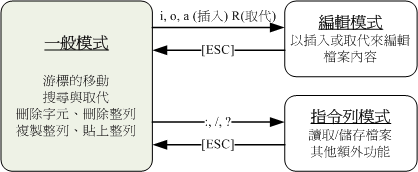
\includegraphics[scale=0.6]{pics/vi-mode} \\
最好用vim命令启动vi, 这个功能更强大一些。上面这个图非常重要,你需要经常点击i,如果进入插入模式,底部会出现--insert--的字样,
否则就是一般模式了。所有的编辑控制(拷贝粘贴等)命令都需要回到一般模式(通过esc来完成。)理解了三个模式, 就可以很好的使用vim了。
	\item common mode \\
	\begin{center}
		\begin{tabular}{c|c}
		\hline
		move & \\
		\hline ctrl+b & previous page\\
		ctrl+f & next page\\
		1G &  begin of document\\
		G & end of document\\
		0& begin of line \\
		\$ & end of line \\
		\hline
		copy & \\
		\hline v & begin to select\\
		y & copy\\
		d & delete\\
		p & paste \\
		yy & copy the whole line \\
		\hline
		delete & \\
		\hline x & delete one\\
		X & delete previous\\
		\hline
		search & \\
		\hline /word & find word\\
		?word & find word previous\\
		n & continue\\
		N & Continue previous\\
		\hline
		\end{tabular}
	\end{center}
	\item command mode \\
	\begin{center}
		\begin{tabular}{c|c}
		\hline :w & write \\
		\hline :q & exit \\
		\hline :! & force (!放到最后)\\
		\hline :n & next document \\
		\hline :N & previous document \\
		\hline :files & show how many files \\
		\hline :sp & 2 windows open files \\
		\hline ctrl+w (release) up arrow & upper window \\
		\hline ctrl+w (release) down arrow& down window \\
		\end{tabular}
	\end{center}

	\end{itemize}




\section{Version Control}
By now,  there is two famous websits, one is code.google.com, the other is github.com. They provides the version control function, and help to manage your source code and documents. the previous one support SVN, the latter one apply git. So, I will introduce these two systems together.
一个最根本的原则,如果单人开发,改动前,必须update, 如果多人开发,除了改动前必须update外,commit前也必须update, (这是因为这个阶段可能别人已经commit了一个新的版本)
\subsection{git}
\subsubsection{basic}
\begin{itemize}
\item 我在github有两个账号,zhaoyan.hrb@gmail.com zhaoyan;yan.zhao.74@gmail.com YanZhao. 有一个项目hello-world,主项目在zhaoyan上,然后我用YanZhao这个账号fork了一下。
zhaoyan上的项目超链接
git://github.com/zhaoyan/hello-world.git(只读版本) git@github.com:zhaoyan/hello-world.git

YanZhao上的项目超链接
git://github.com/YanZhao/hello-world.git(只读版本) git@github.com:YanZhao/hello-world.git


\item The two charactristics about git is \textbf{Distribute} and \textbf{Branch}, Distribute support working offline, Branch can make you manage branch easily and efficiently.
\item \textbf{所有的版本控制,都需要特别注意一个事情,不要取中文的文件名,如果你的英文非常不好,那就用拼音取文件名好了。 这点请务必要注意。}
\item In order to do anything in Git, you have to have a Git repository. This is where Git stores the data for the snapshots you are saving. There are two main ways to get a Git repository. \textbf{One way} is to simply initialize a new one from an existing directory, such as a new project or a project new to source control. \textbf{The second way} is to clone one from a public Git repository, as you would do if you wanted a copy or wanted to work with someone on a project.
\end{itemize}

\subsubsection{github.com}
\begin{itemize}
	\item build a account in github.com \\
		  YanZhao  yan.zhao.74@gmail.com   password for BBS
	\item \linuxcommand{ssh-keygen -t rsa -C yan.zhao.74@gmail.com} \\
        	your public key has been saved in /c/Users/zhao/.ssh/id\_rsa.pub(for windows) ~/.ssh/(for Linux). Then you should paste the public key to the account in github.com. once you finish it, you can use command ssh git@github.com to test it. (github网站上面有更详细的说明。)\\ 你可以把is\_rsa.pub和is\_rsa两个文件拷贝到别的计算机上。这样就不用再另外的计算机上用ssh-keygen命令了。
         	(ssh -v will give you verbose information. you must restart ubuntu after you move id\_rsa to ~/.ssh)。
         

	\item It's a social website, you need to find some friends here and exchange idea. 中国有那些类似的github网站,目前我还不是很清楚。

    \item 有的时候,你看不到项目的超连接地址,可以点击右上角的小眼睛(watchers),也会出现pull request.
    
    \item 完成以上步骤以后,还需要在本地对git进行简单的配置,这样别人才知道你的具体信息,才能和你联系啊。
    
    \begin{verbatim}
	git config --global user.name "zhaoyan"
	git config --global user.email zhaoyan.hrb@gmail.com
	\end{verbatim}
\end{itemize}

\subsubsection{configure}
    \begin{itemize}
    \item windows下,.gitconfig会保存在C:$\backslash$Documents and Settings$\backslash$Administrator下
    \item 运行 git config --global core.editor notepad (在windows下配置成notepad,当热,你也可以选择任何一个你更喜欢的编辑器)
    \item git config --list 可以列出所有的你的配置,你可以进行查看。
    \end{itemize}
    you also can change the ~/.gitconfig file and add below content, it will customize your own git.(color and log alias is more useful)

\begin{verbatim}
[alias]
co = checkout
ci = commit -a
st = status
br = branch
oneline = log --pretty=oneline --since='2 days ago'
onelog = log -p -1
[color]
status = auto
branch = auto
ui = auto
[merge]
tool = kdiff3
[mergetool "kdiff3"]
path = C:/Program Files/KDiff3/kdiff3.exe
keepBackup = false
trustExitCode = false	
\end{verbatim}
    利用KDiff3程序可以利用图形化的程序界面来更改源代码级别上的冲突情况。使用起来也相对简单。\\
编辑.gitignore文件
\begin{verbatim}
# 注释
*.a #忽略所有.a结尾的文件
!lib.a #但是lib.a除外
build/ #忽略build/下所有的文件
doc/*.txt #忽略所有doc/下的文本文件,但是doc/server/arch.txt会包括。
\end{verbatim}

在windows下,安装完成以后,运行git bash命令。可以配置成图形化的diff和merge。其中,下载P4Merge。基本的内容可以参考Pro Git第7章。其中,有一点需要注意,/D/Porgramm$\backslash$ Files/Perforce. 空格前面要加上反斜杠。当你运行git diff以后,就会弹出一个图形界面了。

\subsubsection{把一个已有项目加入到git}
        \begin{verbatim}
		cd test
		git init
		touch README
		git add README
		git add . 
//点代表所有的文件。Directories are added automatically when adding files inside them. That is, directories never have to be added to the repository, and are not tracked on their own. You can say "git add <dir>" and it will add files in there.
		git rm README1 (可以删除一个文件)
		git commit -m "first commit" ( you can't just give empty message)
		git commit -a -m "first commit"
		//这是一种比较简单的写法,综合了add 和commit 两个命令。但是,此处有一点应该注意,那就是git commit -a无法把新增文件或文件夹加入进来,所以,如果你新增了文件或文件夹,那么就要先git add newaddfile,再git commit。针对开发日志,第一行一定要是少于50字的开发概括信息, 而且第二行务必是空行,第三行开始才可以开始细致描述开发信息。 这是因为很多版本服务系统中的email机制都会选取log中的第一行为邮件题目。
		git log //提交完成以后,你可以用log命令检查一下,看看是否已经提交成功了。同时看看过去的历史,也挺有趣的!
        \end{verbatim}
        \textbf{然后,你必须先登陆到github,然后create repository, 名字叫做Other1}
        \begin{verbatim}
		git remote add origin git@github.com:YanZhao/Other1.git
		//origin 其实就是git@github.com:YanZhao/Other1.git的别名,
		git remote show
		//可以查看远端的repository情况。
		git push origin master 	
        //不能省略origin 和master 最好把这个命令写全。master 是默认本地存在的一个分支,你不用显式创建它。
		//这个命令把本地的内容“推”到服务器端。
		//you must have private key file for ssh in those case, you can copy it from ~/.ssh
		\end{verbatim}

\subsubsection{git基本图解}
 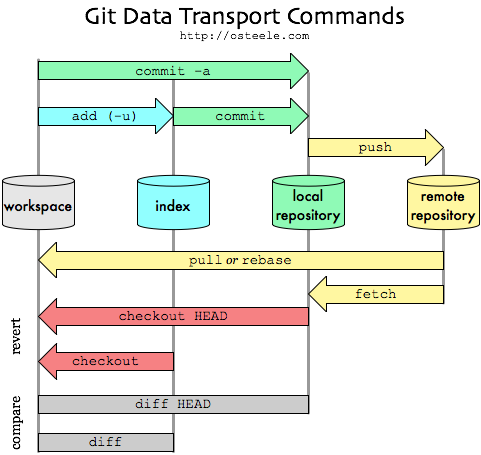
\includegraphics[scale=0.8]{pics/git-transport} \\

\subsubsection{基本命令}
\begin{itemize}
\item status 命令 \\
    这个命令应该算是所有git命令中最常用的一个命令了。应该随时随地的运行它。\par
    git status -s 会给出相对简短的命令,其中有两列,第一列位staging,第二列位working tree。如果你修改了a文件,然后add了,然后又修改了a文件。这个时候,运行git status -s
    会出现 MM a 的标志。具体什么含义,自己去想吧。

\item 提交命令add commit
    \begin{verbatim}
    将 Current working directory 记为 (1)
    将 Index file 记为 (2) 或者叫做 staging
    将 Git repository 记为 (3)

    git add .  //include all untracked file
    git reset -- a.c //从index file中删除掉登记的a.c
    git add -i  //interactive, you can select files to add, 
    select 4[add untraced] first  
    
    git add -u  //not add untracked file

    他们之间的提交层次关系是 (1) -> (2) -> (3)
    git add完成的是(1) -> (2)
    git commit完成的是(2) -> (3)
    git commit -a两者的直接结合

    时间上看,可以认为(1)是最新的代码,(2)比较旧,(3)更旧
    按时间排序就是 (1) <- (2) <- (3)

    此命令将使用当前的暂存区域快照提交。如果刚才提交完没有作任何改动,直接运行此命令的话,相当于有机会重新编辑提交说明,而所提交的文件快照和之前的一样。
启动文本编辑器后,会看到上次提交时的说明,编辑它确认没问题后保存退出,就会使用新的提交说明覆盖刚才失误的提交。
如果刚才提交时忘了暂存某些修改,可以先补上暂存操作,然后再运行 --amend 提交:

    git commit -m 'initial commit'
    git add forgotten_file
    git commit --amend
    \end{verbatim}

\item 文件改名和删除
\begin{verbatim}
rm a
git rm a
git commit -m "delete file a"

git mv a b 等同于mv a b  git rm a  git add b 三个命令
git commit -m "rename a to b"
\end{verbatim}
\item checkout命令
        \begin{verbatim}
git gc //每个月或者每100次commit就运行这个优化历史的程序。
git checkout  //如果没有给文件名,有点类似于(status)命令,只是告诉你一些基本的状态

git checkout . or git checkout file //(update from stage)
git checkout HEAD .  //( update from repo) .代表所有文件。

你可以从多个地方checkout 一个文件,这个有点意识。
git checkout v1.2.3 -- filename
# tag v1.2.3
git checkout stable -- filename
# stable branch
git checkout origin/master -- filename
# upstream master
git checkout HEAD -- filename
# the version from the most recent commit
git checkout HEAD^ -- filename
# the version before the most recent commit
如果你再(1)处更改了代码,你还可以分别从(2)和(3)处或者以上多个地方恢复回来旧的代码。不过你的更改的代码将会永久丢失,
所以以上这些命令要谨慎使用。如果你想保留你的更改。你可以首先:

git add filename 当前更改保存到index
git checkout v1.2.3 filename  得到以前的版本
git diff 比较不同
git checkout filename 再恢复到当前更改。

git checkout HEAD .
# 將所有檔案都 checkout 出來(最後一次 commit 的版本),
注意, 若有修改的檔案都會被還原到上一版. (git checkout -f 亦可)
git checkout xxxx .
# 將所有檔案都 checkout 出來(xxxx commit 的版本, xxxx 是 commit 的編號前四碼), 注意, 若有修改的檔案都會被還原到上一版.
git checkout -- *
# 恢復到上一次 Commit 的狀態(* 改成檔名, 就可以只恢復那個檔案)

\end{verbatim}

\item 比较命令 diff \\
 git fetch 更新以后,你可以利用git diff master origin/master查看一些有哪些改动了。来决定是否你要merge。所以说,fetch+merge比起pull来说更好一些,因为他能停留一下,给你检查一下的机会。 \par
 git diff 的输出中,a代表staging的文件,用-号标注,而b代表working tree的文件,用+号标注。
 \par
    \begin{verbatim}
git diff得到的是从(2)到(1)的变化
git diff –cached得到的是从(3)到(2)的变化
git diff HEAD得到的是从(3)到(1)的变化
git diff tag                    比较tag和HEAD之间的不同。
git diff tag file               比较一个文件在两者之间的不同。
git diff tag1..tag2             比较两个tag之间的不同。
git diff SHA11..SHA12           比较两个提交之间的不同。
git diff tag1 tag2 file or
git diff tag1:file tag2:file    比较一个文件在两个tag之间的不同。

tag可以remote的一个别称,
git remote add xjsff git://github.com/xjsff/hello-world.git
git diff xjsff/master README 查看当前README这个文件与xjsff/master中的README的主要区别。
    \end{verbatim}

\item 远端命令remote \\
\begin{verbatim}
git remote add paul git://github.com/paul/test.git
git remote -v
git remote show paul 显示paul的详细信息,包括分支
git remote rename paul pa
git remote rm pa 删掉pa,因为pa已经不再位项目做贡献了。
\end{verbatim}

\end{itemize}

\subsubsection{history 查看}
\begin{itemize}
\item revision \\
    \begin{verbatim}
    HEAD,FETCH_HEAD,ORIG_HEAD, MERGE_HEAD, COMMIT_EDITMSG:最后一次commit时的提交信息。
    HEAD:表示最近一次的commit。
    MERGE_HEAD:如果是merge产生的commit,那么它表示除HEAD之外的另一个父母分支。
    FETCH_HEAD:使用git-fetch获得的object和ref的信息都存储在这里,这些信息是为日后git-merge准备的。
    HEAD^:表示HEAD父母的信息 等于ORIG_HEAD

    ^ commit对象的第一个父母
    HEAD^^:表示HEAD父母的父母的信息
    HEAD^1:表示HEAD的第一个父母的信息
    HEAD^2:表示HEAD的第二个父母的信息

    ~n commit对象的上溯n代的父母
    HEAD~4:表示HEAD上溯四代的信息,~加数字。

    HEAD:README.txt 代表一个blob对象了。(blob对象的sh-hash值一般看不到,也不方便引用)

    :/fix a bug #代表在commit message 中查找fix a bug有这个串的第一个commit

    @{date specification}
    HEAD@{yesterday}

    git log 后面跟随一个命令集,命名一个集合可以采用一些简写。
    1)B...C #the set of commits that are reachable from either one of r1 or r2 but not from both.
    2)^G D #D的所有父母(包括D),但是不包括G的这个分支。
    3)D F #D,F的所有父母(包括D,F)
    4)C^@ #C的所有父母(不包括C)
    5)
    详细的信息,可以进一步参考gitrevisions命令
    \end{verbatim}

\item blame
    \begin{verbatim}
    git blame -L l2,l3 hello.html
    \\会给出那些行是由那些行提交的。这个信息非常的具体。可以帮你找到元凶to blame。
    \end{verbatim}

\item log
    \begin{verbatim}
    git的历史记录是由一些列相关联的”commit”所组成的。每一次“commit”都会有一个唯一的名称(hash值) 我们可以使用git show再加上hash值显示具体的某次提交。你完全可以用一个最短的且唯一的“名称前几个字符”来只待某次commit:

    git log:显示commit日志
    git log -p:不仅显示commit日志,而且同时显示每次commit的代码改变。
    git log -p -2: 这个命令比较常用,他只显示最近的两次更新。
    git log --oneline 显示简略信息。
    git log --abbrev-commit --pretty=oneline #显示简略的信息
    git log experiment..master #表示的是在master上而不在experiment上的提交。
            a--b--e--f(master)
                \c--d(experiment)
    git log origin/master..HEAD #你将把什么推送到远程。
    git log --left-right master...experiment 显示每个提交属于那一侧的分支。三点代表所有master和experiment分支中的提交。
    \end{verbatim}
\item stash
    \begin{verbatim}
    你正在工作,还么有完成,这个时候,老板让你紧急修改一个release版本的bug,这个时候,stash,然后checkout release. 工作完毕,commit,这个时候git stash pop.

    git stash save “you messaage" #这样可以引入相应的提示信息。
    git stash list #列出所有的stash。
    git statsh pop #如果发生冲突,会自动merge失败。这个时候,需要你手工解决冲突。

    \end{verbatim}
\item show
    \begin{verbatim}
    使用git show加分支名称,亦可以显示分支信息:
    git show master
    git show experimental

    使用HEAD字段可以代表当前分支的头(也就是最近一次commit):
    git show HEAD:README.txt #显示某次提交的README.txt的文件内容。这个时候你不用checkout出来了。
    当然,你也可以重定向到某个文件。例如 git show HEAD:README.txt >OLDREADME.txt文件。
    git show HEAD #同时显示当前提交和上一次提交的差异。
    git show 23df7 (版本号的前五位)
    每一次commit都会有”parent commit”,可以使用^表示parent:
    git show HEAD^ //查看HEAD的父母的信息
    git show HEAD^^ //查看HEAD的父母的父母的信息
    git show HEAD~4 //查看HEAD上溯4代的信息
    要注意的是git-merge是会产生双父母的,这种情况这样处理:
    git show HEAD^1 //查看HEAD的第一个父母
    git show HEAD^2 //查看HEAD的第二个父母


    你可以给复杂名称起个别名:
    git tag V3 5b888 //以后可以用V3来代替复杂的名称(5b888…)
    git show V3
    git branch stable V3 //建立一个基于V3的分支

    可以用git grep帮助我们搜索:
    git grep “print” V3 //在V3中搜索所有的包含print的行
    git grep “print” //在所有的历史记录中搜索包含print的行
    \end{verbatim}
\end{itemize}

\subsubsection{图形界面}
    \begin{itemize}
    \item gitk是一个图形界面程序,你可以查看具体的分支情况。也可以进行一些命令行才能完成的工作。
    \item gitk --all 会列出所有的分支。如果没有--all好像只列出当前的分支。
    you need to understand the basic the meaning of the basic command, so there is a figure below to illustrate it. \\
    \item KDiff3是一个图形化的文件合并工具。使用前需要在.gitconfig文件中进行相关的设置。
    \end{itemize}

\subsubsection{history恢复}
\includegraphics[scale=0.6]{pics/git-history} \\

恢复历史版本: \\
\begin{verbatim}
git commit -C HEAD -a --amend,对最后一次提交做一些修改。(只对最后一次修改有效)
git revert HEAD^^ 会产生一个新的commit。

0)add a,但是发现不想把a置于git控制中,可以用git reset -- a. 
如果已经提交了,可以git rm a. 他会从index file中删除,但是working diretory 中保留a
然后重新提交就可以了。

1)刚刚修改还没有提交
git reset HEAD a.c add了,但没有commit. 取消掉add的内容
git checkout -- a.c  修改了,但是没add,取消掉修改的内容。

2)把某个文件恢复到过去
git checkout HEAD^^ a.c

3)暂时回到过去
git checkout HEAD^^
git chekcout -b dirty
你可以实验,修改等然后
git checkout master

4)永远回到过去
git rest --hard HEAD^^

5)把branch1的历史完全写入到当前的分支当中去。
git rebase branch1
\end{verbatim}



\subsubsection{tag 打标签}
\begin{verbatim}
tag的名字不能包含空格。
建立release branch: git branch RB_1.0
进行一些打包和测试,然后打上标签 git tag 1.0
删掉git branch -D RB_1.0
如果还需要修改这个release, 就
git branch RB_1.01 1.0
git checkout RB_1.01
修改 commit.
git tag 1.01 继续打一个新标签。
git branch -d RB_1.01 删掉这个新的分支。

git archive --format=tar \
--prefix=mysite_release/ \
HEAD | gzip >mysite_relase.tar.gz
//把最后的产品进行打包。
\end{verbatim}


\subsubsection{branch}
分支的的基本命令
\begin{verbatim}
git branch -r 会列出所有remote tracking分支
git branch //会列出当前全部的分支,所在分支会用星号来表示。\\
git branch -D b1 //会删除掉b1这个分支。\\
git checkout branch-name // 切換到 branch-name\\
git checkout -b new-branch master // 從 master 建立新的 new-branch, 並同時切換過去 new-branch\\
git checkout -b newbranch / 由現在的環境為基礎, 建立新的 branch\\
git checkout -b newbranch origin // 於 origin 的基礎, 建立新的 branch\\
git branch -m master mymaster //重命名master为mymaster.(没什么意义) \\
git push origin branch ,//this command will push branch to github. \\
but push branch to server isn't very meaningful, at least I think so. \\
\end{verbatim}

分支的基本知识:\par
1) 主要有两种分支,一种是本地分支,你可以用git branch来查看他们;另外一个就是remote-tracking branches,你可以用git branch -r来查看他们。他们一般的样子类似于:origin/albert和origin/master。你需要注意,origin是源的别名,而不是分支的名字,albert才是真正的分支的名字。\par

2)git push origin experiment \#把一个分支推送到服务器:\\
git push origin local:experiment \#把本地分支改名,推送到服务器端,服务器端分支名为experiment. \\
git push origin :experiment \#把一个分支删除掉,(用空名改名) git push origin erperimental:experimental-by-yan 给remote-tracking-branches另外的名字,这里experimental-by-yan是remote-tracking-branches名字,erperimental是本地分支的名字。 这种方式叫做<source-name>:<destination-name> \par

3)对于remote-tracking branches,你不能直接在上面操作,你可以用git fetch 来 update。或者是与你当前branch merge。或者基于他创建本地分支。\\
git chekcout -b refactored origin/refactored \par
git checkout --track -b refactored origin/refactored (注意有--track).以上两个命令应该大致作用一致。 \par



分支的基本原则:\\
one branch is for (master), one is for merge, the others is for daily experiments. when you want to emerge other's work, you need to build a branch.\\

分支是根据当前的commit 的内容来建立的,而不是根据working tree 或者是index。所以你在merge前,最好先要commit才行。\\

一个分支和主分支merge以后,最后就把它删掉,然后从主分支在创造出一个分支。这样管理起来比较舒服,不要给自己找麻烦。\\

\subsubsection{merge}
分支的合并:\\
\begin{itemize}
\item git merge-base b1 b2 发现b1和b2的共同祖先
\item git cherry -v master test 在master分支中,找到所有test中有但是master中没有的commit.
\item git-merge主要用于将两个或两个以上的开发分支进行合并。主要有三种merge.第一种为straight merge. 他把一个分支的整个历史合并到另外一个分支当中去。还有一种就是squash 把所有的历史变成一个历史commit。 git merge --squash contact。针对于squash,你需要merge以后再提交。最后一种就是cherry-pick,git chekcout master git cherry-pick 321d76f (这是在另外一个分支提交的)。 当然1你也可以git cherry-pick -n 321d76f. -n 告诉git先不提交,然后你就可以继续cherry-pick了。 然后 git commit 不用-m,这个时候一个默认的编辑器就打开了。所有你pick的commit message就会自动出现在那个编辑器中。

\item git merge branchname 用于将branchname分支合并到当前分支中。如果没有冲突,就把分支的commit forward到当前分支中,也就是相当于产生了新的commit。 如果合并发生冲突,需要自己解决冲突)

\item 当merge命令自身无法解决冲突的时候,它会将工作树置于一种特殊的状态,并且给用户提供冲突信息,以期用户可以自己解决这些问题。当然在这个时候,未发生冲突的代码已经被git merge登记在了index file里了。如果你这个时候使用git diff,显示出来的只是发生冲突的代码信息。

在你解决了冲突之前,发生冲突的文件会一直在index file中被标记出来。这个时候,如果你使用git commit提交的话,git会提示:filename.txt needs merge
在发生冲突的时候,如果你使用git status命令,那么会显示出发生冲突的具体信息。\\
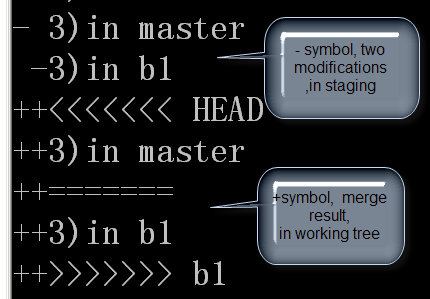
\includegraphics[scale=0.6]{pics/merge-diff} \\

在你解决了冲突之后,你可以使用如下步骤来提交:
第一步:git add filename.txt
第二步:git commit

\item 如果你希望撤销一个分支到merge前的状态,那么使用如下命令:\\
git reset –hard HEAD \\–hard表示将working tree和index file都撤销到以前状态。
Or, if you've already committed the merge that you want to throw away, use this command: git reset --hard ORIG\_HEAD \\
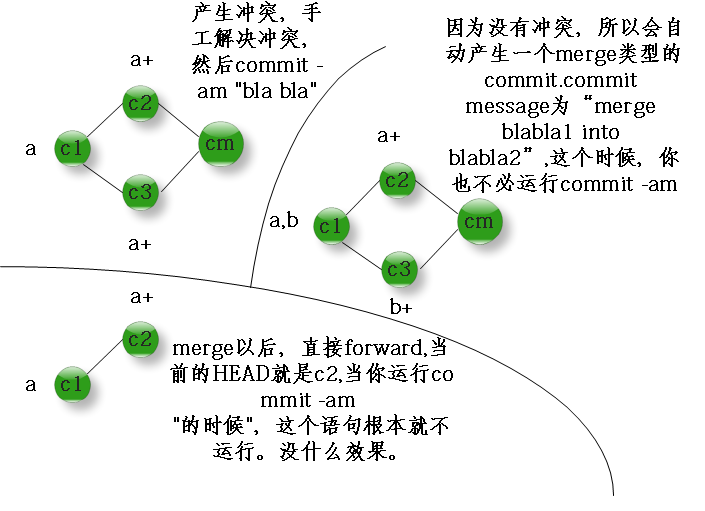
\includegraphics[scale=0.5]{pics/git-merge} \\
\end{itemize}

\subsubsection{reset}
git reset –hard HEAD //–hard表示将working tree和index file都撤销到以前状态。–soft表示只撤销commit,而保留working tree和index file的信息,–mixed会撤销commit和index file,只保留working tree的信息。 这里-mixed是reset的默认选项。

回退掉刚才提交的一个commit. 利用
\begin{verbatim}
git reset -soft HEAD^
\end{verbatim}
git diff返回空,而git diff –cached和git diff HEAD会返回有效信息。这说明使用–soft选项后,只回退了commit的信息,而不会回复到index file一级。哈哈,这就说明了你如果想撤销commit,并且只回退commit的信息,那么就用 -soft吧!

\subsubsection{rebase}
\textbf{Never rebase branches or trees that you pulled. Only rebase local branches. Never ever rebase a branch that you pushed, or that you pulled from another person} \par
rebase的命令和merge的命令有点不太一样。一个标准的流程应该是从master创造出一个分支test,然后在test commit 几次。同时在master commit 几次。这个时候,进入master分支,git rebase test, 或者进入master以后,用merge test, 把test的工作集成到master中去。然后删除test分支。这个就是git的主要工作流程。从这里,你也可以看到 rebase 和merge之间的不同。merge会丢到所有在test分支中的历史。而rebase把这个分支中的历史写道master中了。
 因为他会改变hash的值。可以参考我的网络书签的说明。我一般个人开发,产生一个branch后,master就不变了。 这个时候使用merge 和rebase都是可以的,关键就是你是否对test中的commit的那些历史感兴趣。还有一种流程就是通常 git rebase 1.0

rebase的具体工作流程可以参看这个例子:git rebase test \\
1. 先将test 分支的代码checkout出来,作为工作目录 \\
2. 然后将master分支从test分支创建起的所有改变的补丁,依次打上。如果打补丁的过程没问题,rebase就搞定了 \\
3. 如果打补丁的时候出现了问题,就会提示你处理冲突。处理好了,可以运行git rebase –continue继续直到完成 \\
4. 如果你不想处理,你还是有两个选择,一个是放弃rebase过程(运行git rebase –abort),另一个是直接用test分支的取代当前分支的(git rebase –skip)。 \\

\includegraphics[scale=0.7]{pics/git_rebase} \\

1)如果b是一个本地的branch,如果master上没有m1那么在master 上,执行 git rebase b 和git merge b效果一样,就是增加两个新的commit。 \\

2)如果master 上也有个更新m1。那么需要注意,如果m1只是本地的(你不是pull,同时,你还没有push)同时,你还希望保存
b1 和 b2 两次commit。这个时候,可以使用git rebase b. (因为m1 hash值改变了,所以必须要保证本地化)。\\
3)如果master上m1不是本地化的,那么你最好用merge。但是当你删掉b分支以后,b1,b2消失了。\\

4)如果master上m1不是本地化的,你也可以进入b分支, 然后git rebase master,(不过你需要注意,这个时候,你还在b分支里面。)然后git checkout master , git merge b。
相当于把b当中的b1和b2,放到了m1前面,(m1的hash没变,相当于增加了两个新的commit b1和b2. 你还需要保证b是个本地的branch)
一句话:rebase的使用需要谨慎使用,他的本意是修改历史的作用,如果你没有很明显的理由,就直接用merge好了。\\

rebase branch1 有三个含义,1)当前不再branch1中,2)branch1为焊接接入点,3)当前的分支commit的值改变了。

rebase branch 与rebase master是有区别的。如果你当前在master中,并且以master为主线,那么就应该调用rebase branch。从这个角度上来说,rebase master应该用的不多。除非是上面说的第4种情况,那就是m1已经push出去,并且别人也在用。

rebase两种常用场景,第一就是本地的分支上,两个分支出现并行情况,通过rebase branch1,可以得到相对干净的历史commit. 第二就是rebase thorn/master, 把别人的工作集成到我的master中去,(thorn/master和master都发生了commit)生成一个更干净的历史。他的基本原理和merge大致相同。

\subsubsection{与人合作}
singel person, center control, with branch \\
	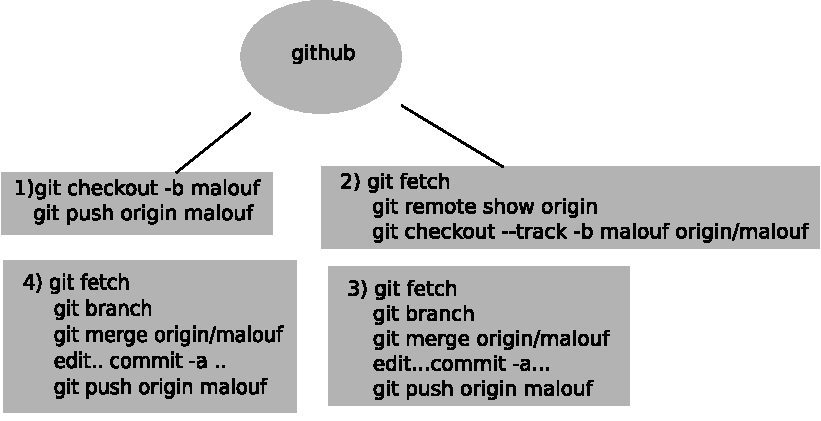
\includegraphics[scale=0.6]{pics/git_branch} \\
   	when you finish the branch, you can merge it with master.

\subsubsection{基于分支合作开发}
\begin{verbatim}
1)git fetch upstream #得到zhaoyan的主线最新开发进展。

2)git checkout -b test_bla upstream/master #以zhaoyan的主线最新开发分支master进展为基础,建立本地的topic分支test_bla (自己想个合适的分支名字,带有描述性。)

3)edit... compile....
   git commit -am "s1"
   edit... compile....
   git commit -am "s2" #你的工作过程可能花费几天,或者几个小时。在这个过程中,upstream/master也许发生了变化,zhaoyan也许在upstream/master提交了新的更新t1。这个时候,commit有以下的历史:

     s1--- s2
____/___t1

4)git fetch upstream #完成你的开发任务以后,你想把你的工作贡献给zhaoyan,这个时候,你需要再次得到zhaoyan的主线最新开发进展。(因为你提交s1和s2的时候,zhaoyan同时在upstream/master上提交了t1)如图。

5a)得到最新的进展以后,你可以使用两种方法,第一种就是利用merge方法。
git merge upstream/master
	如果没有冲突,forward或者自动生成一个merge commit.
	如果有冲突,手工解决你的冲突以后,git commit -am "st1"

     s1--- s2
____/___t1___\st1______


5b)得到最新的进展以后,你可以使用两种方法,第二种就是利用rebase方法。
git rebase upstream/master
	如果没有冲突,forward 或者自动生成一个commit.
	如果有冲突,手工解决你的冲突以后,git add conflict_file 然后git rebase --continue,(不用调用git commit了)。commit历史如下图所示。如果同学们不理解rebase命令的具体含义,请优先选择merge命令。rebase命令具有一定的风险性。

     t1---s1--- s2
____/


6)git push origin test_bla

7)登录到github网站上,找到hello-world项目,切换到test_bla分支。去找那个该死的request pull按钮并点击它。

8)如果zhaoyan已经处理了你的request-pull,并且把你的test_bla集成到zhaoyan的工作中,那么日后,你就可以删掉test_bla这个分支了。git branch -D test_bla

9)git push origin  :test_bla删掉github上的test_bla分支。

10)至此,一个开发流程结束,如果你想开始一个新的开发流程,可以从第1)到9)步重新开始,获得最新进展,重新建立一个新的分支, 完成以后,给zhaoyan发request-pull等等。
\end{verbatim}

\subsubsection{VS2010}


\subsubsection{codeblock}
0)项目文件为pro1.cbp文件,同时,所有源文件也保存到这里,当你编译的时候,会生成两个文件夹
第一个文件夹为bin,第二个文件夹为obj,你可以定义或修改.gitignore文件,加入 bin/ 和obj/。这样在提交的时候就会忽略掉这两个目录。相对来说比较简单。

\subsubsection{kdevelop}
你可以参考如何利用svn,这里重要的不是了解git,而是要理解kdevelop是如何管理一个项目的。\\
0) rm Makefile.in or .svn (if there are) \\
1) go into the src directory, and run git init \\
2) git add * \&\& git commit \\
3) git remote add origin git@github \\
4) git push origin master \\

0) another kdevelop, rm src\\
1) git clone git@github src\\
2) modify Makefile.am with you kdevelop project file.\\
3) in configure dialog, Configure options->linker flager -> add -L./ and add lib to the debug/src directory.\\
4) compile and run.\\

\subsubsection{single person on different computers }
\begin{itemize}
	\item Computer1...
    \begin{verbatim}
    git log HEAD..origin \\查看是否有区别,如果有就fetch,merge。
    git fetch
    git merge origin
    ( git fetch give you more chance to examing it, it's better)
    git commit -a -m " "
    git push
    git log HEAD..origin \\检查是否push成功。
    \end{verbatim}
    \item Computer2...
    \begin{verbatim}
    同样的操作,这里merge的时候,只会产生forword merge,情况相对比较简单。
    \end{verbatim}
\end{itemize}

\subsubsection{cooperation}
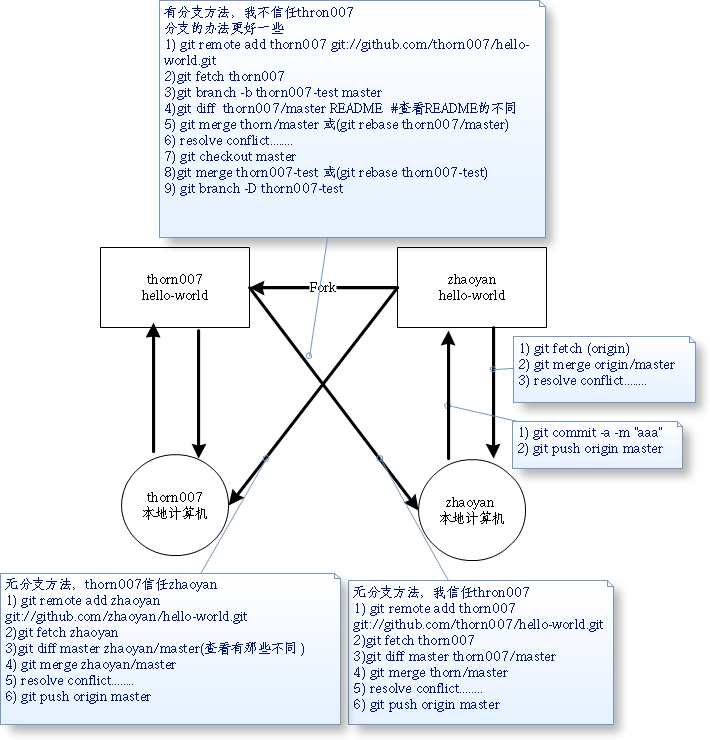
\includegraphics[scale=0.8]{pics/git-corp} \\
\begin{verbatim}
基本命令如下:
git fetch /home/bob/myrepo master:bobworks //用于从bob的工作目录的master分支下载到本地的bobworks分支中。
git-pull的作用就是从一个repository取出内容并合并到另一个repository中。
git pull是git fetch和git merge命令的一个组合。
git pull /home/bob/myrepo 这个命令的意思是从此目录中取出内容并合并到当前分支中。
git pull .就相当于git merge。

下面我给出一个具体的例子:
当合作伙伴bob希望改进我(rocrocket)的工作成果,则:
$git clone /home/rocrocket/project myrepo //此命令用于克隆我的工作到bob的myrepo目录下。请注意,此命令有可能会因为/home/rocrocket的目录权限问题而被拒绝,解决方法是chmod o+rx /home/rocrocket。
(省略bob数小时的开发过程)…
$git commit -a //bob提交自己的改进成果到自己的git仓库中,并口头告知我(rocrocket)他已经完成了工作。

我如果非常信任bob的开发能力:
$ cd /home/rocrocket/project
$ git pull /home/bob/myrepo //pull命令的意思是从远端git仓库中取出(git-fetch)修改的代码,然后合并(git-merge)到我(rocrocket)的项目中去。读者要记住一个小技巧,那就是“git pull .”命令,它和git merge的功能是一样的,以后完全可以用git pull .来代替git merge。请注意,git-pull命令有可能会因为/home/bob的目录权限问题而被拒绝,解决方法是chmod o+rx /home/bob。


如果我不是很信任bob的开发能力:
$ cd /home/rocrocket/project
$ git fetch /home/bob/myrepo master:bobworks //此命令意思是提取出bob修改的代码内容,然后放到我(rocrocket)工作目录下的bobworks分支中。之所以要放到分支中,而不是 master中,就是要我先仔仔细细看看bob的开发成果,如果我觉得满意,我再merge到master中,如果不满意,我完全可以直接git branch -D掉。
$git whatchanged -p master..bobworks //用来查看bob都做了什么
$git checkout master //切换到master分区
$git merge bobworks
$git branch -D bobworks //如果我检查了bob的工作后很不满意,就可以用-D来放弃这个分支就可以了
过了几天,bob如果想继续帮助我开发,他需要先同步一下我这几天的工作成果,只要在其当初clone的myrepo目录下执行git pull即可:
#git pull //不用加任何参数,因为当初clone的时候,git已经记住了我(rocrocket)的工作目录,它会直接找到我的目录来取。
\end{verbatim}

	if modification is small , you can use email+patch; If the modification is big, you can use fork pattern
	\begin{itemize}
    \item you can clone a exist project from other's people or on other computers,
		\begin{verbatim}
		git clone git://github.com/YanZhao/YanZhaoDoc.git
        (this is for visitor clone);
		git clone git@github.com:YanZhao/YanZhaoDoc.git
        (this is for admin clone);
		\end{verbatim}
	\item email topic()
		\begin{verbatim}
		1) git clone http://www.bitsun.com/git/gittutorcn.git
		2) edit and commit
		//method 1 (develop on master)
		$ git  fetch origin
		$ git rebase origin
		$ git for1mat path origin  ->0001-your-buddy-s-contribution.txt
		//method 2 (develop on branche, better)
		$ git checkout -b patch_mubs
		$ git checkout master
		$ git pull
		…
		$ git checkout patch_mubs
		$ git rebase master ( why I need rebase here, I want to know answer)
		
		3)email 0001-your-buddy-s-contribution.txt to vortune@gmail.com
		for vortune:
		1) git checkout -b buddy-in
		2) git am /path/to/0001-your-buddy-s-contribution.txt
		\end{verbatim}
	\end{itemize}

    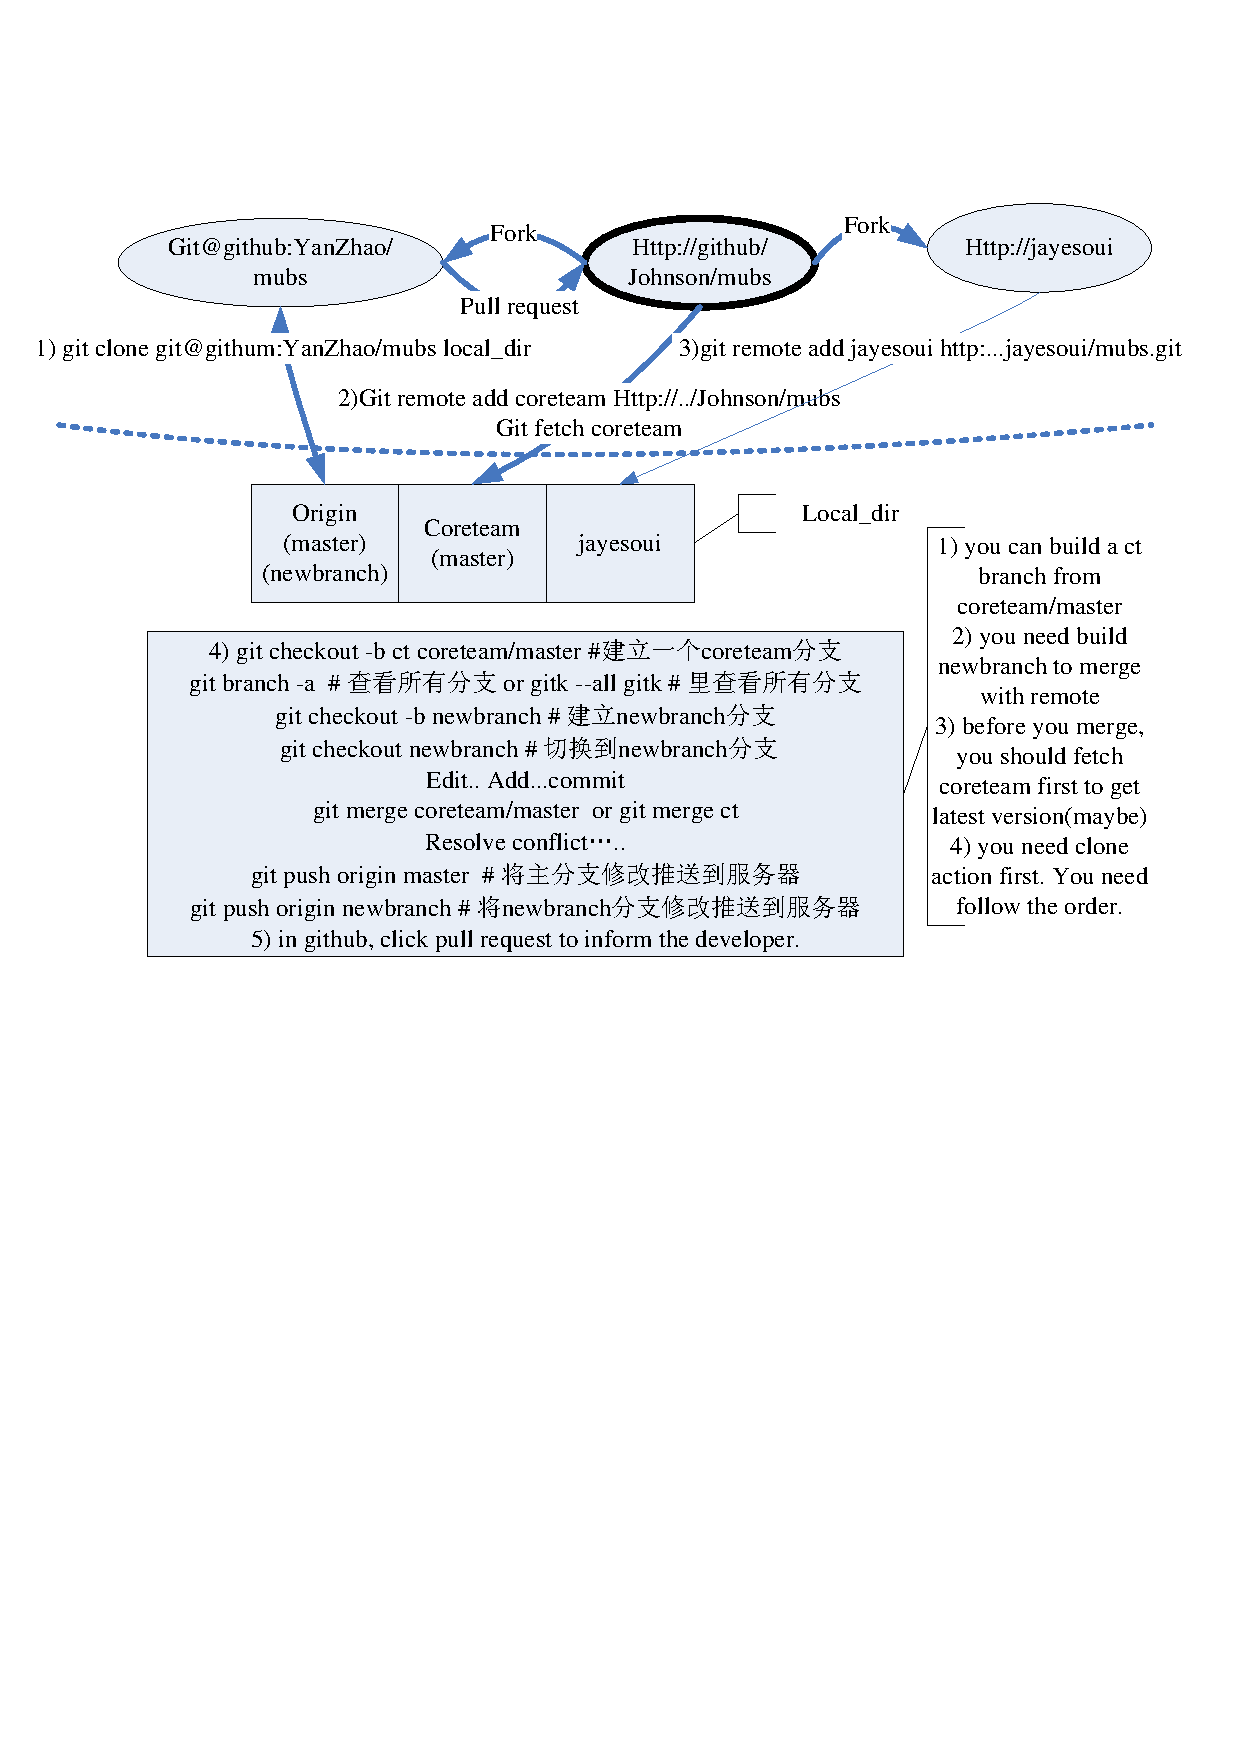
\includegraphics[scale=0.7]{pics/Visio-git_cooperate}

\subsection{SVN}
\subsubsection{basic knowledge}
	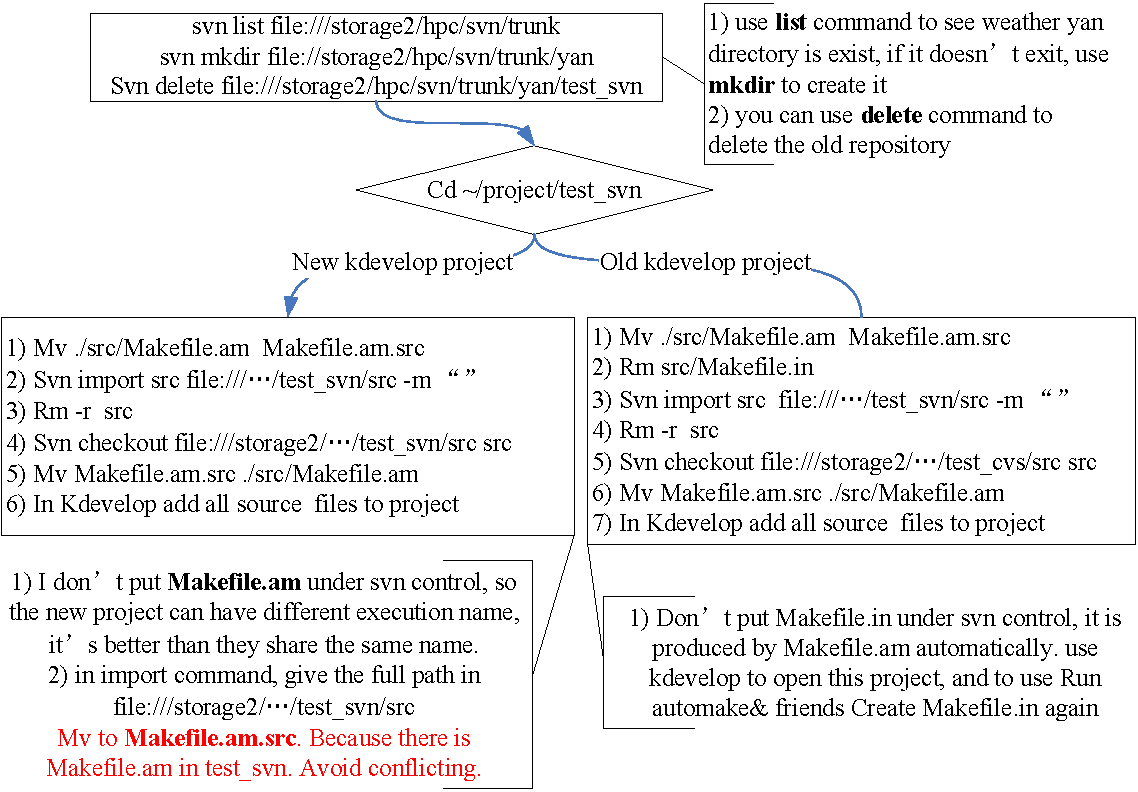
\includegraphics[scale=0.8]{pics/svn1_clip} \\
	 在svn下项目中,我并没有把Makefile.am放到版本控制下,其实,可以把它放到版本控制下, 只不过在新项目中引入的时候,你需要修改Makefile.am中的项目名字,使得他和你的新项目的名字一致就可以了。 \\

	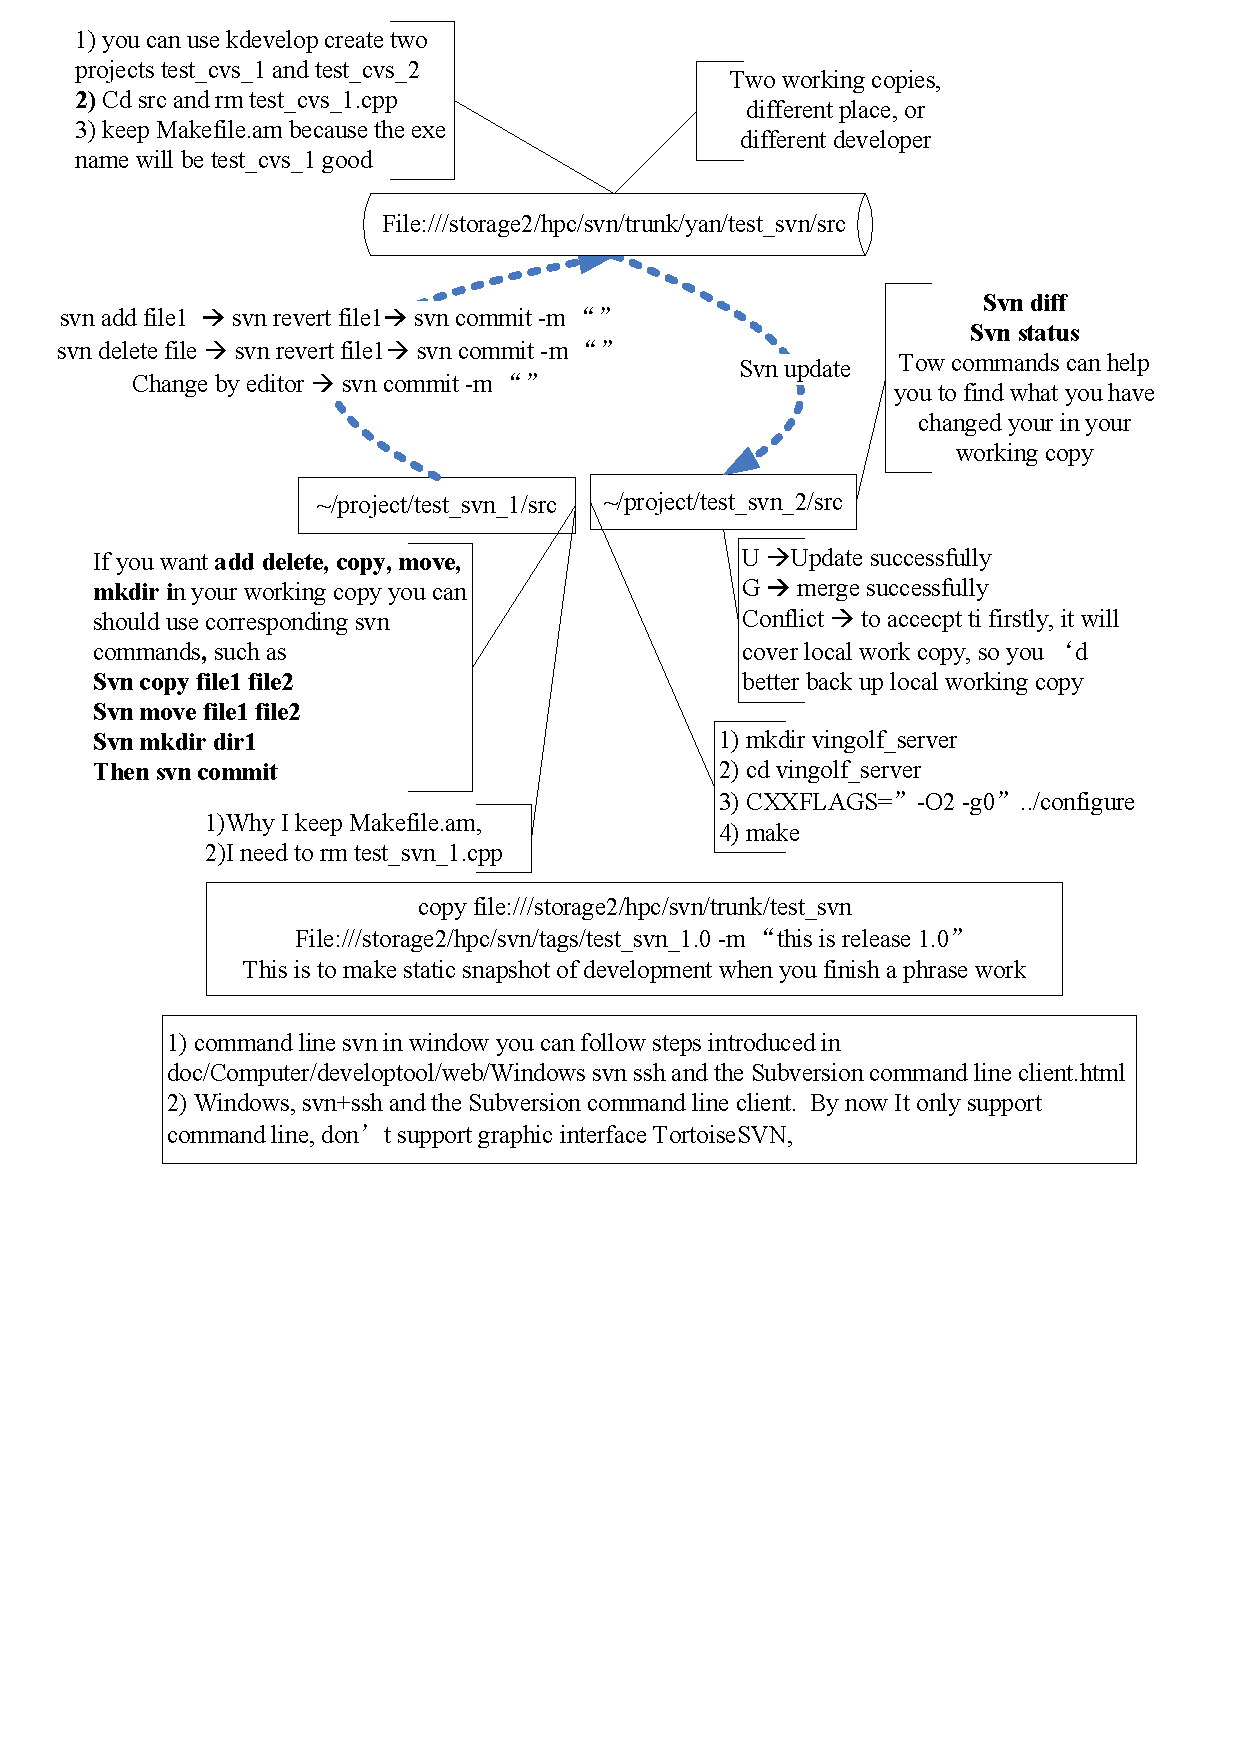
\includegraphics[scale=0.8]{pics/svn2_clip} \\

\subsubsection{common commands}
\begin{enumerate}
 \item update your working copy: \\
   svn update
 \item make changes: \\
    svn add \\
    svn delete dir \\
    svn copy \\
    svn move \\
    svn mkdir dir \\
    svn move src det \\
    svn list :to see which file has been added \\

\item Examing you change: \\
    svn status \\
    svn diff \\
\item undo:
    svn revert \\
\item reslove conflicts: \\
    svn update \\
    svn resolve \\
\item commit: \\
    svn commit \\
\end{enumerate}

\verb=/usr/bin/svn= is the most power tool , you need use it first.

\subsubsection{code.google.com}
\begin{itemize}
    \item svn import  a.file  https://yan-zhao-doc.googlecode.com/svn/trunk/a.file  -m " "
       (you must give the file name in the end of trunk, or it will not work)  \\
	svn import  dir  https://yan-zhao-doc.googlecode.com/svn/trunk/my\_dir  -m " "
	(you can change the dir name  in the end of trunk)
    \item for change: svn checkout https://yan-zhao-doc.googlecode.com/svn/trunk/ yan-zhao-doc --username yan.zhao.74 \\
for other: svn checkout http://yan-zhao-doc.googlecode.com/svn/trunk/ yan-zhao-doc-read-only
    \item  put your mature product in download tab.
\end{itemize}


\subsubsection{merge}
\begin{enumerate}
 \item copy: \\
svn copy http://svn/trunk/   http://svn/branches/new\_feature
\item chekcout:\\
svn checkout
http://svn/branches/new\_feature \\
wokr on new\_feature project with kdevelop
\item merge from trunk:\\
svn merge http://svn/trunk (if trunk is keep running) \\
 (resolve conflict, test, build) \\
svn commit
\item merge from branch:\\
go to trunk workcopy \\
svn merge  --reintegrate http://svn/branches/new\_feature \\
svn commit
\item delte the new feature branch:\\
cd new\_feature \\
svn delete \\
svn commit \\
rm new\_feature
\end{enumerate}

\begin{verbatim}
single merge
0) f:\\temp\\temp (r11)
1) F:\\>svn copy https://yan-zhao-doc.googlecode.com/svn/trunk/
https://yan-zhao-doc.googlecode.com/svn/branches/new\_feature -m "build a new feature\_branch"
( you must use https, not http) (r13)

2) F:\\temp\\>svn co https://yan-zhao-doc.googlecode.com/svn/branches/new\_feature
(it will build new\_feature directory)

3) cd f:\\temp\\new\_feature ->edit-> svn commit ...(r14 ,r15)

svn merge https://yan-zhao-doc.googlecode.com/svn/trunk/
(if trunk is still running)

4) cd f:\\temp\\trunk\\trunk svn merge --reintegrate
https://yan-zhao-doc.googlecode.com/svn/branches/new\_feature

5) svn commit (r16)

6) cd f:\\temp\\new\_feature -> svn delete
https://yan-zhao-doc.googlecode.com/svn/branches/new\_feature (r17)

7) rm f:\\temp\\new\_feature (delete local)
\end{verbatim}
用svn来建立分支和管理分支不是一个好主意,应该使用git。

\subsubsection{How to work under window}
By now commandline client 1.5.5 can work at my vista computer.
run cmd
and run svn co svn+ssh://yzhao@skuld/storage2/hpc/svn/trunk/yan/latex\_doc

\subsubsection{How Working Copies Track the Repository}
For each file in a working directory, Subversion records two essential pieces of information in the .svn/ administrative area:
      what revision your working file is based on (this is called the file's working revision), and
      a timestamp recording when the local copy was last updated by the repository.

Given this information, by talking to the repository, Subversion can tell which of the following four states a working file is in:
\begin{description}
\item[Unchanged, and current]
The file is unchanged in the working directory, and no changes to that file have been committed to the repository since its working revision. An svn commit of the file will do nothing, and an svn update of the file will do nothing.
\item[Locally changed, and current]
The file has been changed in the working directory, and no changes to that file have been committed to the repository since its base revision. There are local changes that have not been committed to the repository, thus an svn commit of the file will succeed in publishing your changes, and an svn update of the file will do nothing.
\item[Unchanged, and out-of-date]
The file has not been changed in the working directory, but it has been changed in the repository. The file should eventually be updated, to make it current with the public revision. An svn commit of the file will do nothing, and an svn update of the file will fold the latest changes into your working copy.
\item[Locally changed, and out-of-date]
The file has been changed both in the working directory, and in the repository. An svn commit of the file will fail with an ``out-of-date'' error. The file should be updated first; an svn update command will attempt to merge the public changes with the local changes. If Subversion can't complete the merge in a plausible way automatically, it leaves it to the user to resolve the conflict.	
\end{description}


\section{sed and awk}
sed is capable of editing task for file, awk is good at some format file and prodcue formate report.
they both can deal with a big file, while with interactive editor may need long time.
\subsection{sed}
	\subsubsection{General Knowledge}
		\begin{itemize}
		\item Firstly, I need to introduce the ed command, It's good start for a lot of useful text tool in linux.
		For example: \linuxcommand{ed test} will open the test file and go to the last line; default, the ed command will only
		be applied to the present line, but both sed and awk will loop all lines in a file. That is the most imporant difference
		in fact, grep means g/re/p command in ed, g means we deal with all lines, and p means print
		\item If there is syntaic error, sed will output command garbled.
		\item both sed awk give default loop for main input of file. It can help you to save some troubles. And they
		also support regular expression. That is two important characteristics when you use these two commands. awk has  two main
		differences with sed. The first one is it provide statements and you can controlthe processing by loop or judge (if..then).
		the second one it support field in a record. Means a word in a line by $1,$2. Sed work on the string level, tr work on the character level. Sed use argument, but tr use <filename.
		And sed can't work on ascII code.
		\item There is three basic displines of sed
			\begin{itemize}
			\item all commands are applied to each line
			\item a command is applied to all lines unless if you use address
			\item you didn't change origanl file, you need redirect to save changed result
			\linuxcommand{sed 's/aa/bb/' oldfile >newfile} then you can use \linuxcommand{diff -y oldfile newfile} to
			check the result.
			\end{itemize}
		\end{itemize}
	\subsubsection{Command Syntax}
	\linuxcommand{sed [options] 'script' file}
		\begin{description}
			\item[Options]: \\
			\begin{tabular}{c|p{0.5\textwidth}}
			\hline
			\op{n} & default, sed will output all lines. n means don't output any thing to the stdout unless you use p command
			For example \linuxcommand{sed -n ``s/old/new/p'' filename} only output those changed lines. \\
			\op{e} & means it followed by a script. When you input more scripts, you need it. \\
			\op{f} & specify the script file\\
			\hline
			\end{tabular}
		\item[Script]
			script is compsed of [address]command, I will introduce below and give some examples.Both [address] and processing can include regex.
			\begin{description}
			\item[Address]:
				\begin{itemize}
				\item a address can be defined by threes way  \\
				
				\[ \textrm{address} \left\{ \begin{array}{l} \textrm{line num, such as 1} \\
						\textrm{a specific character(stand for specific position in a file), such as \$}  \\
						\textrm{regual express,such as /\$/}  \end{array} \right. \]
				
				\item zeor address means deal with all lines
				\item single address means any lines match this address \\
				\linuxcommand{\$d } will delete the last line \\
				\linuxcommand{/\^{}\$/}d \\ empty all the empty lines
				\item a pair of address, means a scope \\
				\linuxcommand{1,\^{} \$d } will delete from a the frist line to the first empty line,
				you can mix three  adress pattern \\
				\linuxcommand{/$\backslash$.TE/,/$\backslash$.TD/d} delete a scope defined by a pair of macors \\
				\end{itemize}
			\item[Commands]: \\
				\begin{enumerate}
				\item replace command
					\begin{description}
					\item[Syntax]: \\
						\begin{itemize}
						\item \linuxcommand{[address]s/pattern/replacement/flags}
						\item \begin{math}
						\textrm{flags} \left\{ \begin{array}{ll}
								\textrm{n} & \textrm{replace nth appearance}  \\
								\textrm{g} & \textrm{global replace}  \\
								\textrm{p} & \textrm{print pattern space} \\
								\textrm{w file} & \textrm{write pattern space to file} \end{array} \right.
						\end{math}
						\\
						\item \[ \textrm{replacement} \left\{ \begin{array}{ll}
								\& & \textrm{use pattern match to replace}  \\
								\textrm{$\backslash$n} & \textrm{match the nth substring}  \\
								\backslash &  \textrm{escape the metacharacter. Guess what $\backslash$ $\backslash$ means?}\\
								\end{array} \right.
						\]
						\end{itemize}
					\item[exmaple]: \\
						\begin{itemize}
						\item /$\backslash$.Ah/\{ \\
							s/$\backslash$.Ah */$\backslash$\Pisymbol{psy}{191} \\
							$\backslash$\Pisymbol{psy}{191} \\
							@A HEAD -/ \\
							s/``//g \\
							 s/\$/$\backslash$\Pisymbol{psy}{191} \\
							\} \\
							a complex example, you use \{ \} to group three commands on the same adress \\
							$\backslash$\Pisymbol{psy}{191} is escpate return, we want to add two empty line
							in front of match line and on emtpy line after it. \\
					
						\item s/ORA/O'Reilly $\backslash$\& Associates/g  It will chanage ORA to O'Reilly ORA Associates
						\item \verb|s/\(.*\):\(.*\)/\2:\1/ change first:second to second:first|
						\item 	sed 's/\^{} [ $\backslash$t]*//;s/[ $\backslash$t]*\$//'  delete all pre and post empty charater \\
							sed 's/foo/bar/'                  replace the first foo \\
							sed 's/foo/bar/4'                 replace the fouth foo \\
							sed 's/foo/bar/g'                 replace all foo to bar \\
							sed 's/$\backslash$(.*$\backslash$)foo$\backslash$(.*foo$\backslash$)/$\backslash$1bar$\backslash$2/'     replace the foo the second from the end \\
							sed 's/$\backslash$(.*$\backslash$)foo/$\backslash$1bar/'             replace the last foo \\
						\item
						\end{itemize}
					\end{description}
				\item delete command
					\begin{description}
					\item[Syntax]: \\
						\begin{itemize}
						\item d is delete command for example: sed '/\^{} \$/d' will delete empty line
						\end{itemize}
					\item[exmaple]: \\
						\begin{itemize}
						\item sed '/\^{} \$/d' will delete empty line
						\end{itemize}
					\end{description}
				\item append,insert,change command
					\begin{description}
					\item[Syntax]: \\
						\begin{itemize}
						\item
						\end{itemize}
					\item[exmaple]: \\
						\begin{itemize}
						\item sed '1,3a\Pisymbol{psy}{191}
							yzhao' filename, it will add three ``yzhao'' at the three lines beginning position.
						\end{itemize}
					\end{description}	
				\item list command
					\begin{description}
					\item[Syntax]: \\
						\begin{itemize}
						\item
						\end{itemize}
					\item[exmaple]: \\
						\begin{itemize}
						\item it can output the pattern space content and use number to represent the invisible character. For example: sed ?n ?e ?l? filename
						\end{itemize}
					\end{description}
				\item y command
					\begin{description}
					\item[Syntax]: \\
						\begin{itemize}
						\item
						\end{itemize}
					\item[exmaple]: \\
						\begin{itemize}
						\item for example sed 'y/abc/xyz/'. It words on character level. Not word conception. Look like tr command
						\end{itemize}
					\end{description}
				\item p command
					\begin{description}
					\item[Syntax]: \\
						\begin{itemize}
						\item
						\end{itemize}
					\item[exmaple]: \\
						\begin{itemize}
						\item If you want to see the middle lines from lines 5 to 10, you can use sed -n '5,10p' /etc/passwd . it?s like awk ?/pattern/?
						\end{itemize}
					\end{description}
				\item q command
					\begin{description}
					\item[Syntax]: \\
						\begin{itemize}
						\item
						\end{itemize}
					\item[exmaple]: \\
						\begin{itemize}
						\item sed ?100q? filename == head ?n 100
						\end{itemize}
					\end{description}
				\item r, w  command
					\begin{description}
					\item[Syntax]: \\
						\begin{itemize}
						\item
						\end{itemize}
					\item[exmaple]: \\
						\begin{itemize}
						\item can read and write to file. It will affect pattern space.
						\end{itemize}
					\end{description}
				
				\end{enumerate}
			\end{description}
		\end{description}
	\subsubsection{Pattern and Hold space}
	There are two important conceptions in sed. Pattern space and hold space.
	command		detail
	Hold	H h	Pattern space ->Hold space
	Get	G g	Hold space-> pattern spac
	Exchange	x	Exchange
	G means append, g means overwrite. They all add a newline symbol at the original content. For example: sed '/\^{} \$/d;G' fileName delete all empty lines and then add empty line.
	%\item before match pattern ``regex''insert a empty line
	sed '/regex/\{x;p;x;\}'
	%\item after match jpattern 'regex' insert a empty line
	sed '/regex/G'
	\subsubsection{Applied Example}
		\begin{itemize}
		\item
		\end{itemize}
	\subsubsection{Note}
		\begin{itemize}
		\item Three different ways to write multi-command in one command line.(when you deal with a big file, It's valueable
		 becuase it only loop the file only once)
			\begin{itemize}
			\item use ; \linuxcommand{sed 's/MA/Mass/;s/PA/Penn/' file}
			\item use \op{e} \linuxcommand{sed -e  's/MA/Mass/' -e 's/PA/Penn/' file}
			\item use \op{f} if there are more than 4 commands and can be used in the later.
			\end{itemize}
		 wait, now I have command \linuxcommand{sed -e 's/pig/cow/g' -e 's/cow/horse/g' file}. what happen? in the end,
		 there is no cow output at all? that is the shortcoming of pattern space. how to resolve it?
		 \linuxcommand{sed -e 's/cow/horse/g' -e 's/pig/cow/g' file} will satisfy you demand.
		 \item for those who want to test this: echo day | sed s/day/night/
		\end{itemize}
\subsection{awk}
Awk think input has structure, line is record and word is field
\subsubsection{Command Syntax}
	\linuxcommand{sed [options] 'script' file}
	\begin{description}
		\item[Options]:
			\begin{itemize}
			\item \op{F} change the delimiter.
			\item \op{f} to specify a scrip file.
			\end{itemize}
		\item[Script]
			script is compsed of [address]\{Statements\}, I will introduce below and give some examples.Both [address] and processing can include regex.
			\begin{description}
			\item[Address]:
				same as inroduction in sed
			\item[Statements]: \\
			\end{description}
		\end{description}
	\subsubsection{Applied Example}
		\begin{itemize}
		\item Awk -F'$\backslash$t' ``\$5\~/MA/ {print \$1, \$2}''  this can give detail information about this command.
		\item In awk, language is included in a pair of \{\}. \{print \$2, \$3\} is different with \{print \$2; print \$3\}. You also can give format information \{print ?\%s \%s?\$2, \$3\}
		\item awk -F$\backslash$| \{print \$1 \$2\} train >train.2
		\item awk -F$\backslash$| \{print \$1 \$2\} train >train.2  awk -F$\backslash$| ``\{printf ``\%s \%s$\backslash$n'', \$1, \$2\} train> train.2 it will provide format information in this formula. Pay
		\item UNIX -> DOS, under this condition, you need to  awk. Because tr can't insert two character to replace one. awk '\{ print \$0``$\backslash$r'' \}' < unixfile > dosfile
		\end{itemize}
	\subsubsection{Note}
		\begin{itemize}
		\item
		\end{itemize}

\section{make}
	\begin{itemize}
		\item Makefile uses compiler and shell programming tools( such as rm, cp etc ) together!
		Make command will look for makefile automatically first. So you should write you own Makefile.
		\item You also can use make –f to specify you own makefile name!
		A Makefile can be regarded as a script file.
		\item The basic part of Makefile is Target: prerequisites
                        tab comm.and
		\item To check which one has changed,  if someone has change, it will call command. That is the most important, you must remember it all the time. And it is not difficult, isn’t it?
		Comment is \#
		\item Make –p to print the default MACRO, \$@ is the names of the file to be made, and \$? Is the names of the changed dependents.
		\item PWD :=\${shell pwd} I need to explain two thing, the first is difference between := and =, := only expand this macro once. PWD is macro. After you define this macro, you can use it later in you paper with \$(PWD)!
		\item @echo can be used to output string. It also can output the variable
		\item use @ to call shell command without output command itself. Use – to tell make to ignore any error.
		\item Make all that is ok, don’t add any other element. Use default to run when you don’t give make and argument
		\item Make –p will list all the default macros
		\item A := \$(wildcard *.a)  ALL\_B :=\$(wildcard *.b)  A\_B :=\$(A:\%.a=\%.b)
		\item First, when you deal with a list of files, you use := ; second when you need aàb you need use A\_B to express this set.
	\end{itemize}

\section{Emacs}
\subsection{General Knowledge}
\[ \left\{ \begin{array}{ccc}
            \textrm{edit mode} & \left\{ \begin{array}{cc} \textrm{buffer 1} & \\ \textrm{buffer 2} & \\ \textrm{buffer 3} & \end{array} \right. & \left\{ \begin{array}{c} \textrm{window 1} \\ \textrm{window 2} \end{array} \right. \\ \\
	    \textrm{dired mode} & \left\{ \begin{array}{c} \textrm{buffer 4}\\ \textrm{buffer 5}  \end{array} \right. & \\
	    \textrm{shell mode} & \ldots & \\
	    \textrm{lang mode} & \ldots & \\
           \end{array}
    \right. \]
You use command to communicate with Emacs. There are five kinds of command.
	\begin{itemize}
	\item C-? : Most common use; ? is any character
	\item M-? : Less common use
	\item C-x C-? : Other commonly used commands
	\item M-x name : You must give name
	\item C-c ? : Command with mode
	\end{itemize}
	
\subsection{edit mode}
this is summmary of shortcut
\[ \left\{ \begin{array}{lll}
            \textrm{move} & \left\{ \begin{array}{ll} \textrm{char} &  \left\{\begin{array}{l} \textrm{forward: Ctrl+f }\\ \textrm{backward:Ctrl+b } \end{array} \right. \vspace{0.5ex} \\
					              \textrm{word} & \left\{\begin{array}{l} \textrm{forward: Alt+f } \\ \textrm{backward:Alt+b } \end{array} \right. \vspace{0.5ex} \\
						      \textrm{line} & \left\{\begin{array}{l} \textrm{begin: Ctrl+a } \\ \textrm{end:Ctrl+e } \end{array} \right.
				     \end{array} \right.  \\ \\
	   \textrm{delete} & \left\{ \begin{array}{ll} \textrm{char} &  \left\{\begin{array}{l} \textrm{forward: backspace } \\ \textrm{backward:Ctrl+d or Del} \end{array} \right.\vspace{0.5ex} \\
					              \textrm{word} & \left\{\begin{array}{l} \textrm{forward: alt+backspace } \\ \textrm{backward:Alt+d } \end{array} \right. \vspace{0.5ex} \\
						      \textrm{line} & \left\{\begin{array}{l} \textrm{whole:Ctrl+k } \\ \textrm{backward:Ctrl+k } \end{array} \right.
				     \end{array} \right.  \\ \\
	   \textrm{select} & \left\{ \begin{array}{ll} \textrm{emacs} &  \left\{\begin{array}{l} \textrm{select: Ctrl+space; move } \\ \textrm{unselect:Ctrl+g} \end{array} \right.\vspace{0.5ex} \\
					              \textrm{other} & \left\{\begin{array}{l} \textrm{select: shift+move }\\ \textrm{select: release shift; move } \end{array} \right. \vspace{0.5ex} \\
				     \end{array} \right.
           \end{array} \right. \]
	   previous short cut come from Emacs, so you can use them directly in Emacs. You can configure the kdevelop and kile with previous shortcut. In this way,
	   you can move cursor without leaving keyboard (that is very valuable) \\
	   Selection seems to be easy in Emacs, you don't need press down shift when you move. but in kile and kdevelop, you need more
\subsubsection{Move command}
\begin{tabular}{|c|c|c|}
\hline
	*Move vertical* & C-p & upward \\ \cline{2-3}
	 & C-n & downword \\
\hline
	*Move character* & C-f or M-j (add sth in .emacs)& forward a character \\ \cline{2-3}
	 & C-b or M-l(add sth in .emacs) & backward a character \\
\hline 	*Move word* & M-f	& forward a word \\ \cline{2-3}
	 & M-b	& Backword a word \\
\hline	*Move line* & C-a & Forward a line \\ \cline{2-3}
 	& C-e	& Backward a line \\
\hline  Move sentence &	M-a	& Forward a sentence \\ \cline{2-3}
	& M-e	& Backward a sentence \\
\hline 	screen	& C-v & 	Up a screen \\ \cline{2-3}
	& M-v	& Down a screen \\
\hline buffer	& M-< & Beginning of buffer\\ \cline{2-3}
	& M-> & End of buffer \\
\hline  other &M-x goto-line& goto-line 	\\
\hline
\end{tabular} \vspace{2ex}\\
You can see the \emph{a,e} means begin and end. \emph{f,b} means forward and backward. 你应该熟悉被*..*标记的那些移动功能,他们一般都比较常用,而且你还不怎么在日常中使用。
Alt is bigger than Ctrl。
\subsubsection{search}
\begin{tabular}{|c|c|}
\hline	Ctrl+s & forward search \\
	Ctrl+r & backward search \\

\hline	Esc Ctrl+s & Regexp forward search \\
	Esc Ctrl+s & Regexp forward search \\
\hline
\end{tabular}\\
Where are you in the document? It's important for you to decide what command to use., if forward fail, try backward at once if you are in the middle of documents

\subsubsection{Delete command}
\begin{tabular}{|c|c|c|}
\hline	undo & C-x u & Undo a deletion one time. (very important) \\
\hline	Undo all & C-y	& Undo all deletion \\
\hline	character	& C-d or del	& Delete next \\ \cline{2-3}
	& backspace & Delete previous \\
\hline	Word & M-d & Delete next word \\ \cline{2-3}
	& M-Del & Delete previous word \\
\hline	line	& C-k & \\
\hline	sentence & M-k &	\\
\hline	block	& C-W &	\\
\hline
\end{tabular} \\
*** M-b M-d delete whole word C-a C-k delete whole line

\subsubsection{Mark}
\begin{tabular}{|c|c|}
\hline C-space	& mark\\
\hline C-w & cut\\
\hline M-w & copy\\
\hline C-y & paste\\
\hline
\end{tabular} \\
M-x hexl-mode

\subsection{lang mode}

\subsubsection{perl}
\begin{itemize}
 \item Debug a perl programme, you can input M-x perldb
 \item S   is step
 \item b [line] insert a breakpoint
 \item r run until meet a breakpoint
\end{itemize}

\subsection{shell mode}
\begin{tabular}{|p{0.1\textwidth}|c|c|}
\hline M-! & Run shell command once & \\
\hline M-x & M-p & Previous command \\ \cline{2-3}
	& M-n & Next command\\ \cline{2-3}
	& C-c C-z & Ctrl +z\\ \cline{2-3}
	& C-c C-d & Ctrl +d\\ \cline{2-3}
	& c-c C-c & Ctrl +c\\ \cline{2-3}
	& C-c C-r & The first line\\ \cline{2-3}
	& C-c C-e & The last line\\ \cline{2-3}
\hline
\end{tabular} \\
在mc中,你可以直接切换到控制台,在应用上更方便一些。

\subsection{dired mode}
\begin{tabular}{|c|c|}
\hline C-x d & Come in Dired\\
\hline D & delete\\
\hline X & execute\\
\hline G & refresh\\
\hline M & mark\\
\hline V & \\
\hline \% & \\
\hline C & Copy\\
\hline R & Rename\\
\hline
\end{tabular}


\subsection{buffer}
\begin{tabular}{|c|c|}
\hline C-x C-q & Mark it read only \\
\hline C-x C-f & Produce a file\\
\hline C-x b & Will display most recently disappeared\\
\hline C-x C-b &  Buffer list (q exist buffer list)\\
\hline C-x k & Kill a buffer\\
\hline
\end{tabular}

\subsection{window}
\begin{tabular}{|c|c|}
\hline C-x 2   or   M-2	& V 2 windows \\
\hline C-x 3   & H 2 windows\\
\hline C-x 4 b  & Produce a new window(buffer)\\
\hline C-x 4 f & Produce a new window(file)\\
\hline C-x 0   or    M-0 & Kill present\\
\hline C-x 1   or    M-1 (only one) & Keep present\\
\hline C-x o   or   M-o &  Change to other window\\
\hline
\end{tabular} \\
\subsection{online help}
There are three kind of help information:
	\begin{itemize}
	\item online help! This is the first step you should learn\\
		\begin{tabular}{|c|c|}
		\hline C-h c & Describe key briefly( you must click key) \\
		\hline C-h b & Describe corresponding buffer help(that is useful) \\
		\hline C-h k & Describe key ( you must click key following)\\
		\hline C-h f & Describe funciton\\
		\hline C-h I & See the last 100 key stroke\\
		\hline C-h r & Read manual \\
		\hline C-h v & Describe variable( give variable name)\\
		\hline C-h m& Describe mode( tell the current buffer mode)\\
		\hline C-x C-h& It will give all key binding beginning with C-x\\
		\hline C-h b &  is very useful! You can use if more often. \\
		\hline
		\end{tabular}
	\item If you know the exact name, you can use above method, but if you don't know the exact name, you can use apropos (C-h a) and apropos-command. And give your description, it will list all command or variables in the help file. 7
	\item type ? when you in these commands
		\begin{itemize}
		\item dired (C-x d) \\
			You see a list of the most frequently used commands in the minibuffer. This list is far from complete. Type C-h m (for describe-mode) for more comprehensive documentation and C-h b (for describe-bindings) for all
 the key bindings available to you.
		\item list-buffers (C-x C-b) \\
			ou see a *Help* window giving information on buffer menu mode. This command has the same effect as typing C-h m (for describe-mode).
		\item save-some-buffers (C-x s) \\
			Behavior is similar to query-replace just described.
		\item query-replace (M-\%)  \\
		You see a *Help* window listing the available commands. Typing C-h does the same thing. This also works with query-replace-regexp.
		\end{itemize}
	\end{itemize}
\subsection{summary}
目前,我已经学习了vim,mc,emacs。我个人主要是使用mc,集成了文件管理和相应的编辑工作。这一点上与emacs 有点重复。对于轻量级别的编辑工作,我应该学习使用vim.所以说,对emacs来说,如果你要编写perl并且调试他, 或者如果你要一个文档有两个窗口显示,(做一些比较工作)。只有这个时候,我才考虑使用emacs程序。



\ifx \allfiles \undefined
\end{CJK*}
\end{document}
\fi
